% This is samplepaper.tex, a sample chapter demonstrating the
% LLNCS macro package for Springer Computer Science proceedings;
% Version 2.20 of 2017/10/04
%
\documentclass[runningheads,final]{llncs}
%
%\documentclass[runningheads]{llncs}

%\setlength{\paperheight}{232.8mm}
%\setlength{\paperwidth}{151.5mm}
%\setlength\voffset     {-23mm}
%\setlength\hoffset     {-34mm}


\usepackage{hyperref}
\usepackage[framemethod=TikZ]{mdframed}
\usepackage{multicol}
\usepackage{xcolor}
\usepackage[final]{changes}
\usepackage{graphicx}
\usepackage{url}
\usepackage{amsmath}
\usepackage{bm}
\usepackage{multirow}
\usepackage{enumitem}
\usepackage{tcolorbox}
\usepackage{booktabs}
\usepackage{tabularx}
\usepackage{rotating}
\usepackage{subfig}
\usepackage{latexsym,amssymb,amsmath}

\usepackage{makecell}
\usepackage{xspace}
%\usepackage{times}
%\usepackage[obeyFinal]{todonotes}

\usepackage{scalerel}
\usepackage[ruled,noend]{algorithm2e}
\usepackage{paralist}
\usepackage{wrapfig}
\usepackage{adjustbox}

%%%%%%%%%%%%%%%%%%%%%%%%%%%%%%%%%%%%%%%%%%%%%%%%%%%%%%%%%%%%%%%%%%%%%%%%%%%%%%
%%% Time-stamp: "2018-09-07 18:35:03 calvanese"
%%%%%%%%%%%%%%%%%%%%%%%%%%%%%%%%%%%%%%%%%%%%%%%%%%%%%%%%%%%%%%%%%%%%%%%%%%%%%%

%%%%%%%%%%%%%%%%%%%%%%%%%% General Math

\newcommand{\A}{\ensuremath{\mathcal{A}}}
\newcommand{\B}{\ensuremath{\mathcal{B}}}
%\newcommand{\C}{\ensuremath{\mathcal{C}}}
\newcommand{\D}{\ensuremath{\mathcal{D}}}
\newcommand{\E}{\ensuremath{\mathcal{E}}}
\newcommand{\F}{\ensuremath{\mathcal{F}}}
%\newcommand{\G}{\ensuremath{\mathcal{G}}}
\renewcommand{\H}{\ensuremath{\mathcal{H}}}
\newcommand{\I}{\ensuremath{\mathcal{I}}}
\newcommand{\J}{\ensuremath{\mathcal{J}}}
\newcommand{\K}{\ensuremath{\mathcal{K}}}
\renewcommand{\L}{\ensuremath{\mathcal{L}}}
\newcommand{\M}{\ensuremath{\mathcal{M}}}
\newcommand{\N}{\ensuremath{\mathcal{N}}}
\renewcommand{\O}{\ensuremath{\mathcal{O}}}
\renewcommand{\P}{\ensuremath{\mathcal{P}}}
\newcommand{\Q}{\ensuremath{\mathcal{Q}}}
\newcommand{\R}{\ensuremath{\mathcal{R}}}
%\renewcommand{\S}{\ensuremath{\mathcal{S}}}
\newcommand{\T}{\ensuremath{\mathcal{T}}}
%\newcommand{\U}{\ensuremath{\mathcal{U}}}
\newcommand{\V}{\ensuremath{\mathcal{V}}}
\newcommand{\W}{\ensuremath{\mathcal{W}}}
\newcommand{\X}{\ensuremath{\mathcal{X}}}
\newcommand{\Y}{\ensuremath{\mathcal{Y}}}
\newcommand{\Z}{\ensuremath{\mathcal{Z}}}

%%%%%%%%%%%%%%%%%%%%%%%%%% Abbreviations

%%\newcommand{\eset}{\emptyset}
%%\newcommand{\col}{\colon}
\newcommand{\ol}[1]{\overline{#1}}                % overline
%\newcommand{\ul}[1]{\underline{#1}}               % underline
%%\newcommand{\uls}[1]{\underline{\raisebox{0pt}[0pt][0.45ex]{}#1}}
%% ul with space between text and line

\newcommand{\ra}{\rightarrow}
\newcommand{\Ra}{\Rightarrow}
\newcommand{\la}{\leftarrow}
\newcommand{\La}{\Leftarrow}
%\newcommand{\lra}{\leftrightarrow}
\newcommand{\Lra}{\Leftrightarrow}
\newcommand{\lora}{\longrightarrow}
\newcommand{\Lora}{\Longrightarrow}
\newcommand{\lola}{\longleftarrow}
\newcommand{\Lola}{\Longleftarrow}
\newcommand{\lolra}{\longleftrightarrow}
\newcommand{\Lolra}{\Longleftrightarrow}
%\newcommand{\ua}{\uparrow}
\newcommand{\Ua}{\Uparrow}
\newcommand{\da}{\downarrow}
\newcommand{\Da}{\Downarrow}
\newcommand{\uda}{\updownarrow}
\newcommand{\Uda}{\Updownarrow}

%%%%%%%%%%%%%%%%%%%%%%%%%% Relations

%%\newcommand{\incl}{\subseteq}
%%\newcommand{\imp}{\rightarrow}
\newcommand{\per}{\mbox{\bf .}}                  % period

%%%%%%%%%%%%%%%%%%%%%%%%%% Delimiters

%%\newcommand{\quotes}[1]{{\lq\lq #1\rq\rq}}
%\newcommand{\set}[1]{\{#1\}}                      % set
%\newcommand{\Set}[1]{\left\{#1\right\}}
\newcommand{\bigset}[1]{\Bigl\{#1\Bigr\}}
\newcommand{\bigmid}{\Big|}
\newcommand{\size}[1]{|{#1}|}                     % cardinality of a set
%%\newcommand{\Card}[1]{\left| #1\right|}
\newcommand{\card}[1]{\sharp #1}
\newcommand{\tup}[1]{\langle #1\rangle}            % tuple
\newcommand{\Tup}[1]{\Braket{#1}}
\newcommand{\norm}[2]{\|#1\|_{#2}}
\newcommand{\setone}[2][1]{\set{#1\cld #2}}

%%%%%%%%%%%%%%%%%%%%%%%%%% STYLING AND SPACING

%\newcommand{\inlinetitle}[1]{\smallskip\noindent\textbf{#1.}\xspace}





\newcolumntype{C}{>{\centering\arraybackslash}X}

%\makeatletter
%\g@addto@macro\normalsize{%
%\setlength{\abovecaptionskip}{-2pt}
%\setlength{\belowcaptionskip}{12pt}
%\setlength\abovedisplayskip{3pt}
%\setlength\belowdisplayskip{3pt}
%\setlength\abovedisplayshortskip{3pt}
%\setlength\belowdisplayshortskip{3pt}
%}
%\makeatother

\newcounter{dummy} 
\newcounter{dummy1} 
\newcounter{dummy2}
\newcounter{dummy3} 
\newcounter{dummy4}
\newcounter{dummy5} 
\newcounter{dummy6}
\newcounter{dummy7}
%\numberwithin{dummy}{section}

\usepackage[thmmarks,amsmath]{ntheorem}
%\theorempreskip{1pt}
%\theorempostskip{1pt}

%\theoremstyle{plain}
%\theorembodyfont{\normalfont}
%\theoremseparator{.}
%\let\definition\relax
%\theoremsymbol{\ensuremath{\square}}
%\newtheorem{definition}{Definition}


\let\proposition\relax
\let\theorem\relax
\let\lemma\relax
\let\definition\relax
\theoremseparator{.}
\theorembodyfont{\itshape}
\theoremsymbol{$\triangleleft$}
\newtheorem{theorem}[dummy]{Theorem}
\newtheorem{lemma}[dummy1]{Lemma}
\newtheorem{definition}[dummy2]{Definition}
\newtheorem{proposition}[dummy3]{Proposition}

\let\remark\relax
\let\example\relax
%\let\example*\relax
\theorembodyfont{\normalfont}
\newtheorem{example}[dummy4]{Example}
\newtheorem{remark}[dummy5]{Remark}
%\newtheorem{example*}[dummy4]{Example}


\theoremstyle{nonumberplain}
\theoremheaderfont{\itshape}
\theorembodyfont{\normalfont}
\let\proof\relax
\theoremseparator{.}
\theoremsymbol{\ensuremath{\dashv}}
\newtheorem{proof}[dummy6]{Proof}


\qedsymbol{\ensuremath{\dashv}}


%%% Local Variables:
%%% mode: latex
%%% TeX-master: "main"
%%% save-place: t
%%% End:

\usepackage{tkz-graph}
\usetikzlibrary{matrix,automata,arrows,calc,fit}
\usetikzlibrary{decorations.pathreplacing,positioning}


\definecolor{deepblue}{HTML}{0C3B80}
\definecolor{deepgreen}{HTML}{2EA601}
%\definecolor{deepblue}{HTML}{232F3E}
%\definecolor{chaptercolor}{HTML}{232F3E}{0.8}
\definecolor{lightOrange}{HTML}{FFA03C}
\definecolor{darkOrange}{HTML}{F1800A}
\definecolor{lightBlue}{HTML}{0174CD}
\definecolor{greenF}{HTML}{2CBB5C}
\definecolor{cyan}{HTML}{86A6D5}
\definecolor{darkred}{HTML}{8B0000}

\usetikzlibrary{automata,positioning}
\usetikzlibrary{arrows}
\usetikzlibrary{decorations.markings}
\usetikzlibrary{shapes.misc, positioning}
\usetikzlibrary{arrows.meta,decorations.markings}



%%%%%%%%%%%%%%%%%%%%% TIKZS MACROS
\def\DTZU {2ex}

\tikzstyle{taskfg} = [
  text=deepblue,
]

\tikzstyle{taskbg} = [
  fill=cyan!50,
]

\tikzstyle{taskline} = [
  draw=deepblue,
]

\tikzstyle{taskstyle} = [
  ultra thick,
  taskfg,
  taskbg,
  taskline
]

\tikzstyle{task} = [
  rectangle,
  minimum width=12mm,
  minimum height=10mm,
  taskstyle
]

\tikzstyle{smalltask} = [
  rectangle,
  minimum width=8mm,
  minimum height=6mm,
  taskstyle,
  very thick
]

\tikzstyle{constraint} = [
  ultra thick,
  taskline,
  taskbg
]

\tikzstyle{response} = [
  constraint,
  *-triangle 60
]

\tikzstyle{precedence} = [
  constraint,
  *triangle 60-
]
\tikzstyle{succession} = [
  constraint,
  *triangle 60-*
]


\tikzstyle{respondedexistence} = [
  constraint,
  *-
]

\tikzstyle{coexistence} = [
  constraint,
  *-*
]

\tikzstyle{negationconstraint} = [
  constraint,
  postaction={decorate,decoration={markings,
   mark=at position .5 with {\arrow[xshift=0.15*\DTZU]{Bar[width=1.5*\DTZU]}},
   mark=at position .5 with {\arrow[xshift=-0.15*\DTZU]{Bar[width=1.5*\DTZU]}}
  }}
]

\tikzstyle{notcoexistence} = [
  negationconstraint,
  coexistence,
]

\tikzstyle{negationresponse} = [
  constraint,
  response,
  postaction={decorate,decoration={markings,
   mark=at position .5 with {\arrow[xshift=0.15*\DTZU]{Bar[width=1.5*\DTZU]}},
   mark=at position .5 with {\arrow[xshift=-0.15*\DTZU]{Bar[width=1.5*\DTZU]}}
  }}
]

\tikzstyle{negationsuccession} = [
  constraint,
  succession,
  postaction={decorate,decoration={markings,
   mark=at position .65 with {\arrow[xshift=0.15*\DTZU]{Bar[width=1.5*\DTZU]}},
   mark=at position .65 with {\arrow[xshift=-0.15*\DTZU]{Bar[width=1.5*\DTZU]}}
  }}
]



\tikzstyle{exclusivechoice} = [
  constraint,
  -,
  postaction={decorate,decoration={markings,
   mark=at position .5 with {\arrow[xshift=0.5*\DTZU]{Diamond[width=1*\DTZU]}} 
  }}
]

\tikzstyle{choice} = [
  constraint,
  -,
  postaction={decorate,decoration={markings,
   mark=at position .5 with {\arrow[xshift=0.5*\DTZU]{Diamond[width=1*\DTZU]}},
    mark=at position .5 with {\arrow[xshift=0.28*\DTZU,white,scale=.6]{Diamond[width=1*\DTZU]}} 
  }}
]







\tikzstyle{circ} = [
  solid,
  text=black
]

\tikzstyle{timeline} = [
  -,
  thin,
  ]
  
\tikzstyle{snapshot} = [
  -,
  thin,
  densely dotted,
  ]
  

\tikzstyle{objnode} = [
  inner sep=2pt,
  circle,
  ultra thick,
]

\tikzstyle{tobj} = [
  objnode,
  taskfg,
  taskbg,
  taskline
]

\tikzstyle{cobj} = [
  objnode,
  classfg,
  classbg,
  classline
]

\tikzstyle{link} = [
  solid,
  -angle 60
]
%%%%%%%%%%%%%%%%%%%%%
\newcommand{\LTL}{\ensuremath{\text{LTL}}\xspace}
\newcommand{\LTLf}{\ensuremath{\text{LTL}_f}\xspace}
\newcommand{\PLTL}{\ensuremath{\text{PLTL}_f}\xspace}
\newcommand{\PLTLz}{\ensuremath{\text{PLTL}_f^0}\xspace}

\newcommand{\Wuntil}{\mathcal{W}}

\newcommand{\At}{\ensuremath{\mathsf{At}}\xspace}

\newcommand{\nats}{\ensuremath{\mathbb{N}}\xspace}
\newcommand{\acc}{\ensuremath{\mathsf{acc}}\xspace}
\newcommand{\branch}{\ensuremath{\mathsf{b}}\xspace}
\newcommand{\exa}{\ensuremath{\mathsf{exa}}\xspace}
\newcommand{\ini}{\ensuremath{\mathsf{in}}\xspace}
\newcommand{\ms}{\ensuremath{\mathsf{m}}\xspace}
\newcommand{\wt}{\ensuremath{\mathsf{wt}}\xspace}
\newcommand{\run}{\ensuremath{\mathsf{run}}\xspace}
\newcommand{\rnk}{\ensuremath{\mathsf{rk}}\xspace}
\newcommand{\swt}{\ensuremath{\mathsf{w}}\xspace}
\newcommand{\csub}{\ensuremath{\mathsf{csub}}\xspace}
\newcommand{\END}{\ensuremath{\mathsf{END}}\xspace}

\newcommand{\atom}{\ensuremath{\mathbf{a}}\xspace}

\newcommand{\Amc}{\ensuremath{\mathcal{A}}\xspace}
\newcommand{\Bmc}{\ensuremath{\mathcal{B}}\xspace}
\newcommand{\Imc}{\ensuremath{\mathcal{I}}\xspace}
\newcommand{\Lmc}{\ensuremath{\mathcal{L}}\xspace}
\newcommand{\Omc}{\ensuremath{\mathcal{O}}\xspace}
\newcommand{\Pmc}{\ensuremath{\mathcal{P}}\xspace}
\newcommand{\Qmc}{\ensuremath{\mathcal{Q}}\xspace}
\newcommand{\Smc}{\ensuremath{\mathcal{S}}\xspace}
\newcommand{\Wmc}{\ensuremath{\mathcal{W}}\xspace}

\newcommand{\Imf}{\ensuremath{\mathfrak{I}}\xspace}

\newcommand{\PS}{\text{\sc{PSpace}}\xspace}
\newcommand{\ET}{\text{\sc{ExpTime}}\xspace}

\newcommand{\prob}[1]{\ensuremath{\scaleobj{1.2}{\circledcirc}_{#1}}\xspace}

\newcommand{\argmax}{\text{argmax}\xspace}
\newcommand{\declare}{Declare\xspace}
\newcommand{\pdeclare}{ProbDeclare\xspace}
\newcommand{\constraint}[1]{\texttt{#1}}
\newcommand{\activity}[1]{\ensuremath{\mathsf{#1}}}
%\newtheorem{theorem}{Theorem}
%\newtheorem{lemma}[theorem]{Lemma}
%\newtheorem{claim}[theorem]{Claim}
%\newtheorem{proposition}[theorem]{Proposition}
%\newtheorem{corollary}[theorem]{Corollary}
%\theoremstyle{definition}
%\newtheorem{example}[theorem]{Example}
%\newtheorem{definition}[theorem]{Definition}



%% temporal operators
\newcommand{\Next}{{\ensuremath\raisebox{0.25ex}{\text{\scriptsize$\bigcirc$}}}}
\newcommand{\Until}{\ensuremath{\mathbin{\mathcal{U}}}}
\newcommand{\Wntil}{\ensuremath{\mathbin{\mathcal{W}}}}









\allowdisplaybreaks

%%%%%%%%%%%%%%%%%%%%%%%%%%%%%
%%%%%%%  Conference / arXiv Versions  %%%%%%%
\newif\iffull\fulltrue
%\fullfalse		%%% uncomment to make conference version
\newcommand{\FullT}[1]{\iffull #1 \fi}
\newcommand{\FullF}[1]{\iffull \else #1 \fi}
\newcommand{\FullTF}[2]{\iffull #1 \else #2 \fi}
\usepackage{tkz-graph}
\usetikzlibrary{matrix,automata,arrows,calc,fit}
\usetikzlibrary{decorations.pathreplacing,positioning}


\definecolor{deepblue}{HTML}{0C3B80}
\definecolor{deepgreen}{HTML}{2EA601}
%\definecolor{deepblue}{HTML}{232F3E}
%\definecolor{chaptercolor}{HTML}{232F3E}{0.8}
\definecolor{lightOrange}{HTML}{FFA03C}
\definecolor{darkOrange}{HTML}{F1800A}
\definecolor{lightBlue}{HTML}{0174CD}
\definecolor{greenF}{HTML}{2CBB5C}
\definecolor{cyan}{HTML}{86A6D5}
\definecolor{darkred}{HTML}{8B0000}

\usetikzlibrary{automata,positioning}
\usetikzlibrary{arrows}
\usetikzlibrary{decorations.markings}
\usetikzlibrary{shapes.misc, positioning}
\usetikzlibrary{arrows.meta,decorations.markings}



%%%%%%%%%%%%%%%%%%%%% TIKZS MACROS
\def\DTZU {2ex}

\tikzstyle{taskfg} = [
  text=deepblue,
]

\tikzstyle{taskbg} = [
  fill=cyan!50,
]

\tikzstyle{taskline} = [
  draw=deepblue,
]

\tikzstyle{taskstyle} = [
  ultra thick,
  taskfg,
  taskbg,
  taskline
]

\tikzstyle{task} = [
  rectangle,
  minimum width=12mm,
  minimum height=10mm,
  taskstyle
]

\tikzstyle{smalltask} = [
  rectangle,
  minimum width=8mm,
  minimum height=6mm,
  taskstyle,
  very thick
]

\tikzstyle{constraint} = [
  ultra thick,
  taskline,
  taskbg
]

\tikzstyle{response} = [
  constraint,
  *-triangle 60
]

\tikzstyle{precedence} = [
  constraint,
  *triangle 60-
]
\tikzstyle{succession} = [
  constraint,
  *triangle 60-*
]


\tikzstyle{respondedexistence} = [
  constraint,
  *-
]

\tikzstyle{coexistence} = [
  constraint,
  *-*
]

\tikzstyle{negationconstraint} = [
  constraint,
  postaction={decorate,decoration={markings,
   mark=at position .5 with {\arrow[xshift=0.15*\DTZU]{Bar[width=1.5*\DTZU]}},
   mark=at position .5 with {\arrow[xshift=-0.15*\DTZU]{Bar[width=1.5*\DTZU]}}
  }}
]

\tikzstyle{notcoexistence} = [
  negationconstraint,
  coexistence,
]

\tikzstyle{negationresponse} = [
  constraint,
  response,
  postaction={decorate,decoration={markings,
   mark=at position .5 with {\arrow[xshift=0.15*\DTZU]{Bar[width=1.5*\DTZU]}},
   mark=at position .5 with {\arrow[xshift=-0.15*\DTZU]{Bar[width=1.5*\DTZU]}}
  }}
]

\tikzstyle{negationsuccession} = [
  constraint,
  succession,
  postaction={decorate,decoration={markings,
   mark=at position .65 with {\arrow[xshift=0.15*\DTZU]{Bar[width=1.5*\DTZU]}},
   mark=at position .65 with {\arrow[xshift=-0.15*\DTZU]{Bar[width=1.5*\DTZU]}}
  }}
]



\tikzstyle{exclusivechoice} = [
  constraint,
  -,
  postaction={decorate,decoration={markings,
   mark=at position .5 with {\arrow[xshift=0.5*\DTZU]{Diamond[width=1*\DTZU]}} 
  }}
]

\tikzstyle{choice} = [
  constraint,
  -,
  postaction={decorate,decoration={markings,
   mark=at position .5 with {\arrow[xshift=0.5*\DTZU]{Diamond[width=1*\DTZU]}},
    mark=at position .5 with {\arrow[xshift=0.28*\DTZU,white,scale=.6]{Diamond[width=1*\DTZU]}} 
  }}
]







\tikzstyle{circ} = [
  solid,
  text=black
]

\tikzstyle{timeline} = [
  -,
  thin,
  ]
  
\tikzstyle{snapshot} = [
  -,
  thin,
  densely dotted,
  ]
  

\tikzstyle{objnode} = [
  inner sep=2pt,
  circle,
  ultra thick,
]

\tikzstyle{tobj} = [
  objnode,
  taskfg,
  taskbg,
  taskline
]

\tikzstyle{cobj} = [
  objnode,
  classfg,
  classbg,
  classline
]

\tikzstyle{link} = [
  solid,
  -angle 60
]
%%%%%%%%%%%%%%%%%%%%%

\makeatletter
\g@addto@macro\normalsize{%
\setlength{\abovecaptionskip}{0pt}
\setlength{\belowcaptionskip}{-10pt}
\setlength\abovedisplayskip{3pt}
\setlength\belowdisplayskip{3pt}
\setlength\abovedisplayshortskip{3pt}
\setlength\belowdisplayshortskip{3pt}
}
\makeatother

\theorempreskip{2pt}
\theorempostskip{2pt}

%%%%%%%%%%%%%%%%%%%%%%%%%%%%%






\newcommand*\circled[1]{\tikz[baseline=(char.base)]{
            \node[shape=circle,draw,inner sep=2pt] (char) {#1};}}


\newcommand{\nodedist}{6mm}
\newcommand{\textsize}{80mm}
\newcommand{\taskdist}{12mm}
\newcommand{\autshift}{5mm}

\tikzstyle{pconstraint} = [
  draw=lightBlue!80,
]

\tikzstyle{pwords} = [
  text=lightBlue!80
]

\newcommand{\exclose}{\ensuremath{\Diamond \activity{close}}}
\newcommand{\negexclose}{\ensuremath{\neg \Diamond \activity{close}}}


\sloppy
\begin{document}
%
\title{Probabilistic Trace Alignment}
%\subtitle{\emph{Vision Paper}}
%
%\titlerunning{Abbreviated paper title}
% If the paper title is too long for the running head, you can set
% an abbreviated paper title here
%
\author{
Giacomo Bergami \and
Fabrizio Maria Maggi \and
Marco Montali\inst{1} \and
Rafael Pe\~naloza\inst{2}}

\authorrunning{F.M.~Maggi et al.}
% First names are abbreviated in the running head.
% If there are more than two authors, 'et al.' is used.
%
\institute{
Free University of Bozen-Bolzano, Italy \\\email{\{maggi,montali\}@inf.unibz.it}
\and
University of Milano-Bicocca \\\email{rafael.penaloza@unimib.it}
}

%\vspace{1.5cm}
%
%
\maketitle              % typeset the header of the contribution
%\linespread{0.98}
%\vspace{-0.5cm}

\begin{abstract}
\end{abstract}

\keywords{Declarative Process Models, Probabilistic Temporal Logics, Conformance Checking}

%
%
%%

%\section{Introduction}
\label{introduction}

Temporal business constraints have been extensively adopted to declaratively capture the acceptable courses of execution in a business process. In particular, the \emph{\declare} constraint-based process modeling language \cite{PeSV07} has been introduced as a front-end language to specify business constraints based on Linear Temporal Logic over finite traces (\LTLf) \cite{DeVa13}.

In general, business constraints are interpreted logically in a crisp way.
 This means that an execution trace conforms with a constraint model if all the constraints therein are satisfied. This is too restrictive when one wants to capture patterns that recur in many application domains, such as:
 \begin{compactitem}[$\bullet$]
 \item best practices, captured as constraints that should hold in the majority, but not necessary all cases (example: an order is shipped via truck in $90\%$ of the cases);
 \item outlier behaviors, i.e., constraints that only apply to very few cases that should still considered to be conforming (example: an order is shipped via car in less than $1\%$ of the cases);
 \item constraints involving activities that are not all necessarily controlled by the organization that orchestrates the process, and for which only some guarantees can be given about their proper executability (example: whenever an order is accepted, payment is performed by the customer in $8$ cases out of $10$).
 \end{compactitem}

Surprisingly enough, to the best of our knowledge no attempt has been done, so far, to make constraint-based process modeling approaches able to capture this form of uncertainty. In this paper, we tackle this timely and important challenge, relying on recent results on probabilistic temporal logics over finite traces \cite{MaMP20}. Specifically, \emph{we equip business constraints with a natural, probabilistic notion of uncertainty based on the ratio of traces in a log that must satisfy the constraint}, and use the resulting probabilistic constraints to lift \declare\ to its probabilistic variant that we call \pdeclare.
We then discuss the semantic implications of this approach, showing how it has to combine logical and probabilistic reasoning to tackle the semantics of probabilistic constraints and their interplay.
We finally show how this combined reasoning can be applied to verify the consistency of a \pdeclare model, do conformance checking, and carry out probabilistic constraint entailment, i.e., estimate with which probability a \pdeclare model implies a given \LTLf formula.

\endinput
A key functionality that any process-aware information system should support is that of {\it monitoring} \cite{DBLP:journals/is/LyMMRA15}. Monitoring concerns the ability to verify at runtime whether an actual process execution conforms with a prescriptive business process model. This runtime form of conformance checking is instrumental to detect, and then suitably handle, deviations appearing in ongoing process instances.

A common way of representing monitoring requirements that capture the expected behavior prescribed by a process model is by using declarative, business constraints. Many studies demonstrated that, in several settings, business constraints can be formalized in terms of temporal logic rules \cite{MPVC11}.
Within this paradigm, the \emph{\declare} constraint-based process modeling language \cite{PeSV07} has been introduced as a front-end language to specify business constraints based on Linear Temporal Logic over finite traces (\LTLf) \cite{DeVa13}. The advantage of this approach is that the automata-theoretic characterization of \LTLf is based on standard, finite-state automata. These can be exploited to provide advanced monitoring facilities where the state of constraints is determined in a sophisticated way by combining the events collected at runtime with the possible, future continuations \cite{MMWV11,DDGM14}, in turn enabling the early detection of conflicting constraints \cite{MWMV11}.


In a variety of application domains, business constraints are inherently \emph{uncertain}. This is clearly the case for constraints which:
\begin{inparaenum}[\it (i)]
\item capture best practices that have to be followed by default, i.e., in most, but not necessarily all, cases;
\item link controllable activities to activities that are under the responsibility of uncontrollable, external stakeholders;
\item should hold in exceptional but still conforming courses of execution.
 \end{inparaenum}
 Uncertainty is intrinsically present also when business constraints are discovered from event data. It is then very surprising that only very few approaches incorporate uncertainty as a first-class citizen. This is the case not just when the prescriptive behavior to be monitored is expressed as a set of business constraints, but also when a more conventional imperative approach is adopted \cite{DBLP:conf/bpm/LeemansSA19}.


It is well known that combining uncertainty with temporal logics is extremely challenging. This is due to the interplay of temporal operators and uncertainty, which becomes especially tricky considering that, usually, temporal logics are interpreted over infinite traces. The resulting, combined logics then come with semantic or syntactic restrictions (see, e.g., \cite{Ognj06,KovP18}).
To tackle these issues, the probabilistic temporal logic over finite traces $\PLTL$, and its fragment $\PLTLz$, have been recently proposed in \cite{MaMP20}. Since these logics are defined over finite traces, they are the natural candidate to enrich existing constraint-based process modeling approaches with uncertainty.

In this paper, we indeed employ $\PLTLz$ to achieve this goal.  Specifically, we exploit the fact that $\PLTLz$ handles time and probabilities in a way that naturally matches with the notion of conformance: a constraint $\varphi$ holds with probability $p$ if, by considering all the traces contained in a log, $\varphi$ is satisfied by fraction $p$ of all the traces contained therein. Based on this observation, we provide a threefold contribution.

First, we exploit $\PLTLz$ to introduce \emph{probabilistic constraints} and delve into their semantics and conceptual meaning; notably, our semantics is based on the already established notion of stochastic language \cite{DBLP:conf/bpm/LeemansSA19}. We then show how probabilistic constraints can be used to naturally lift the \declare language to its probabilistic version \pdeclare.
%
Second, we observe that probabilistic Declare constraints can be discovered off-the-shelf using already existing techniques for declarative process discovery \cite{LMMR07,MaCV12,CiccioM15,DBLP:conf/caise/SchonigRCJM16}, with strong guarantees on the consistency of the generated models. In fact, the discovered constraints are for sure (probabilistically) consistent, without incurring in the notorious consistency issues experienced when the discovered constraints are interpreted in a crisp way \cite{DMMM17}.
%
 Third, we study how to monitor probabilistic constraints,  where constraints and their combinations may be in multiple monitoring states at the same time, though with different associated probabilities. This is based on the fact that a single \pdeclare model gives raise to multiple scenarios, each with its own distinct probability, where some of the constraints are expected to be satisfied, and the others to be violated. Specifically, we show how to lift existing automata-theoretic monitoring techniques to this more sophisticated probabilistic setting, and report on a proof-of-concept implementation of the resulting framework.

The paper is structured as follows. After preliminary notions introduced in Section~\ref{sec:preliminaries}, we introduce the syntax and semantics of probabilistic constraints in Section~\ref{sec:probdeclare}. In Section~\ref{sec:discovery}, we discuss how \pdeclare constraints can be discovered from event data using existing techniques. In Section~\ref{sec:monitoring}, we show how to monitor probabilistic constraints, and report on the corresponding implementation.



%\newcommand{\length}{\mathit{length}}
\newcommand{\true}{\mathit{true}}
\newcommand{\false}{\mathit{false}}
\newcommand{\aut}{\mathcal{A}}
\newcommand{\tasks}{\Sigma}
\newcommand{\trace}{\tau}

\newcommand{\close}{\activity{close}}
\newcommand{\accept}{\activity{accept}}
\newcommand{\reject}{\activity{reject}}

\section{LTL over Finite Traces and the Declare Framework}
\label{sec:preliminaries}
As a formal basis for specifying crisp (temporal) business constraints, we adopt the customary choice of Linear Temporal Logic over finite traces (\LTLf \cite{DeVa13,DDGM14}). This logic is at the basis of the well-known \declare \cite{PeSV07} constraint-based process modeling language.
We provide here a gentle introduction to this logic and to the \declare framework.

\subsection{Linear Temporal Logic over Finite Traces}

$\LTLf$ has exactly the same syntax as standard $\LTL$, but, differently from $\LTL$, it interprets formulae over an unbounded, yet finite linear sequence of states. Given an alphabet $\Sigma$ of atomic propositions (in our setting, representing activities), an \LTLf formula $\varphi$ is built by extending propositional logic with temporal operators:
\[\varphi ::= a \mid \lnot \varphi \mid \varphi_1\lor \varphi_2
 \mid \Next\varphi \mid \varphi_1\Until\varphi_2 \quad \text{ where $a \in \Sigma$.}\]


%The semantics of \LTLf is given in terms of \emph{finite traces}
%denoting finite, \emph{possibly empty}, sequences
%$\tau=\tau_0,\ldots,\tau_n$ of elements from the alphabet $\Sigma$. The evaluation of a formula is done in a given state (i.e., position) of the trace.


The semantics of \LTLf is given in terms of \emph{finite traces} denoting finite, \emph{possibly empty} sequences $\tau=\tup{\tau_0, \ldots, \tau_n}$ of elements of $2^\Sigma$, containing all possible propositional interpretations of the propositional symbols in $\Sigma$. In the context of this paper, consistently with the literature on business process execution traces, we make the simplifying assumption that in each point of the sequence, one and only one element from $\Sigma$ holds. Under this assumption, $\tau$ becomes a total sequence of activity occurrences from $\Sigma$, matching the standard notion of (process) execution trace. We indicate with $\tasks^*$ the set of all traces over $\tasks$. The evaluation of a formula is done in a given state (i.e., position) of the trace, and we use the notation $\tau,i\models \varphi$ to express that $\varphi$ holds in the position $i$ of $\tau$. We also use $\tau \models \varphi$ as a shortcut notation for $\tau,0\models\varphi$. This denotes that $\varphi$ holds over the entire trace $\tau$ starting from the very beginning and, consequently, logically captures the notion of \emph{conformance} of $\tau$ against $\varphi$. We also say that $\varphi$ is \emph{satisfiable} if it admits at least one conforming trace.

%We start by giving an intuitive account of the resulting semantics. In the syntax above, operator $\Next$ denotes the \emph{next state} operator, and $\Next \varphi$ is true if $\varphi$ is true is true now if there exists a next state (i.e., the current state is not at the end of the trace), and in the next state $\varphi$ holds. Operator $\Until$ instead is the \emph{until} operator, and $\varphi_1\Until\varphi_2$ is true if $\varphi_1$ holds now and continues to hold until eventually, in a future state, $\varphi_2$ holds. From the given syntax we can derive the usual boolean operators $\land$ and $\rightarrow$, the two formulae $\true$ and $\false$, as well also additional temporal operators. We consider in particular the following three:
%\begin{compactitem}[$\bullet$]
%\item (eventually) $\Diamond \varphi = \true \Until \varphi$ is true if there is a future state where $\varphi$ holds;
%\item (globally) $\Box \varphi = \neg \Diamond \neg \varphi$ is true if now and in all future sates $\varphi$ holds;
%\item (weak until) $\varphi_1 \Wntil \varphi_2 = \varphi_1\Until\varphi_2 \lor \Box \varphi_1$ relaxes the until operator by admitting the possibility that $\varphi_2$ never becomes true, in this case by requiring that is true if $\varphi_1$ holds now and in all future states.
%\end{compactitem}
% To define the semantics formally, we denote the length of trace $\tau$ as $\length(\tau) =  n+1$.


In the syntax above, operator $\Next$ denotes the \emph{next state} operator, and $\Next \varphi$ is true if there exists a next state (i.e., the current state is not at the end of the trace), and in the next state $\varphi$ holds. Operator $\Until$ instead is the \emph{until} operator, and $\varphi_1\Until\varphi_2$ is true if $\varphi_1$ holds now and continues to hold until eventually, in a future state, $\varphi_2$ holds. From these operators, we can derive the usual boolean operators $\land$ and $\rightarrow$, the two formulae $\true$ and $\false$, as well as additional temporal operators. We consider, in particular, the following three:
\begin{compactitem}[$\bullet$]
\item (eventually) $\Diamond \varphi = \true \Until \varphi$ is true if there is a future state where $\varphi$ holds;
\item (globally) $\Box \varphi = \neg \Diamond \neg \varphi$ is true if now and in all future states $\varphi$ holds;
\item (weak until) $\varphi_1 \Wntil \varphi_2 = \varphi_1\Until\varphi_2 \lor \Box \varphi_1$ relaxes the until operator by admitting the possibility that $\varphi_2$ never becomes true, in this case by requiring that $\varphi_1$ holds now and in all future states.
\end{compactitem}
%We write $\tau \models \varphi$ as a shortcut notation for $\tau,0\models \varphi$, and say that formula $\varphi$ is \emph{satisfiable}, if there exists a trace $\tau$ such that $\tau \models \varphi$.

\begin{example}
The $\LTLf$ formula $\Box(\activity{accept} \rightarrow \Diamond\activity{pay})$ models that, whenever an order is accepted, then it is eventually paid. The structure of the formula follows what is called \emph{response template} in \declare.
\end{example}

%Every $\LTLf$ formula $\varphi$ can be translated into a corresponding standard finite-state automaton $\aut_\varphi$ that accepts all and only those finite traces that satisfy $\varphi$ \cite{DeVa13,DDGM14}. Although the complexity of reasoning with $\LTLf$ is the same as that of $\LTL$, finite-state automata are much easier to manipulate in comparison with B\"uchi automata, which are necessary when formulae are interpreted over infinite traces.

\subsection{Declare}
\begin{table}[t]
\caption{Some \declare templates, their textual and graphical representation, the corresponding \LTLf formalization and the \LTLf formula capturing their complement (i.e., their logical negation).
\label{tab:constraints}}
\centering
\begin{adjustbox}{width=0.9\textwidth,center}
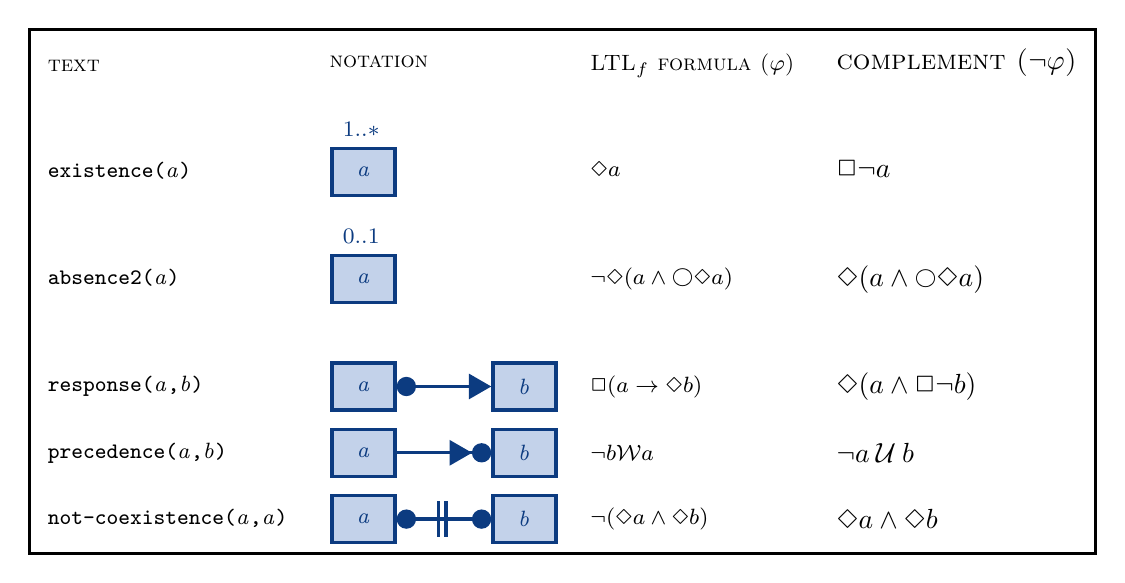
\begin{tikzpicture}
  \matrix[  nodes={node distance=\nodedist,minimum height=6mm},
            rectangle, draw,
            nodes in empty cells,
            row sep=2mm,column sep=3mm,
            very thick,
            column 1/.style={anchor=west,font=\footnotesize},
            column 2/.style={anchor=west,xshift=1mm,font=\footnotesize},
            column 3/.style={anchor=west,xshift=1mm,font=\footnotesize},
            column 4/.style={anchor=west},
            >=latex,->,
          ] (declarematrix) {
    \node {\textsc{text}};
    &
    \node[yshift=.5mm] {\textsc{notation}};
  &
    \node {\textsc{\LTLf\ formula ($\varphi$)}};
    &
    \node[yshift=.5mm] {\textsc{complement ($\neg\varphi$)}};
    \\
    \node {
      \begin{tabular}{@{}l@{}}
      \constraint{existence($\mathit{a}$)} \\
      \end{tabular}
    };
    &
    \node[smalltask,xshift=1.5mm] (a) {$\mathit{a}$};
    \node[taskfg,above=-1mm of a,xshift=-.3mm]{\footnotesize $1..\ast$};
    &
    \node {$\Diamond {a}$};
    &
    \node {$\Box \neg {a}$};

    \\
     \node {
      \begin{tabular}{@{}l@{}}
        \constraint{absence2($\mathit{a}$)}\\
      \end{tabular}
    };
    &
    \node[smalltask,xshift=1.5mm] (a) {$\mathit{a}$};
    \node[taskfg,above=-1mm of a,xshift=-.3mm]{\footnotesize $0..1$};

    &
    \node {$\neg \Diamond ({a} \land \Next \Diamond {a})$};
    &
    \node {$\Diamond ({a} \land \Next \Diamond {a})$};
    \\
    \node {
      \begin{tabular}{@{}l@{}}
        \constraint{response($\mathit{a}$,$\mathit{b}$)}
      \end{tabular}
    };
    &
    \node[smalltask,xshift=1.5mm] (a) {$\mathit{a}$};
    \node[above=-1mm of a,xshift=-.3mm]{\footnotesize $~$};
    \node[smalltask,right=\taskdist of a] (b) {$\mathit{b}$};
    \path[response,very thick] (a) -- (b);
    &
    \node {$\Box ({a} \rightarrow \Diamond {b})$};
    &
    \node {$\Diamond ({a} \land \Box \neg {b})$};
    \\
    \node {
      \begin{tabular}{@{}l@{}}
        \constraint{precedence($\mathit{a}$,$\mathit{b}$)}\\
      \end{tabular}
    };
    &
    \node[smalltask,xshift=1.5mm] (a) {$\mathit{a}$};
    \node[smalltask,right=\taskdist of a] (b) {$\mathit{b}$};
    \path[precedence,very thick] (b) -- (a);
    &
    \node {$\neg {b} \Wuntil {a}$};
    &
    \node {$\neg {a} \Until {b}$};
    \\
    \node {
      \begin{tabular}{@{}l@{}}
        \constraint{not-coexistence($\mathit{a}$,$\mathit{a}$)}\\

      \end{tabular}
    };
    &
    \node[smalltask,xshift=1.5mm] (a) {$\mathit{a}$};
    \node[smalltask,right=\taskdist of a] (b) {$\mathit{b}$};
    \path[notcoexistence,very thick] (a) -- (b);
    &
    \node {$\neg(\Diamond {a} \land \Diamond {b})$};
    &
    \node {$\Diamond {a} \land \Diamond {b}$};
    \\
%    \node {
%      \begin{tabular}{@{}l@{}}
%        \constraint{neg-response(\activity{a},\activity{b})}\\
%        $\Box( \activity{a} \limp \neg \bigcirc\Diamond \activity{b})$
%      \end{tabular}
%    };
%    &
%    \node[smalltask,xshift=1.5mm] (a) {\activity{a}};
%    \node[smalltask,right=\taskdist of a] (b) {\activity{b}};
%    \path[negationresponse,very thick] (a) -- (b);
%    \\
    };
\end{tikzpicture}
\end{adjustbox}
\end{table} 
\declare\ \cite{PeSV07} is a declarative process modeling language based on \LTLf. More specifically, a \declare model fixes a set of activities, and a set of constraints over such activities, formalized using \LTLf formulae. The overall model is then formalized as the conjunction of the \LTLf formulae of its constraints.

Among all possible \LTLf formulae, \declare selects some pre-defined patterns. Each pattern is represented as a \declare template, i.e., a formula with placeholders to be substituted by concrete activities to obtain a constraint. Constraints and templates have a graphical representation; Table~\ref{tab:constraints} lists the \declare templates used in this paper. A \declare model is then graphically represented by showing its activities, and the application of templates to such activities (which indicates how the template placeholders have to be substituted to obtain the corresponding constraint).

%Automata-based techniques for $\LTLf$ have been adopted to tackle fundamental tasks within the lifecycle of \declare processes, such as consistency checking \cite{PeSV07,MPVC11}, enactment and monitoring \cite{PeSV07,MMWV11,DDGM14}, and discovery support \cite{MaCV12}.




\begin{example}
\label{ex:inconsistency}
Consider the following \declare model, constituting a (failed) attempt of capturing a fragment of an order-to-shipment process:

\begin{center}
  \resizebox{3.2cm}{!}{
        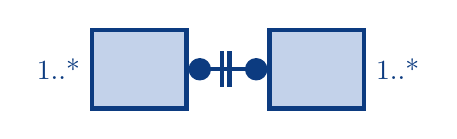
\begin{tikzpicture}
        \node[task] (accept) {\accept};
        \node[task,right=of accept] (reject) {\reject};
        \node[left=0mm of accept,taskfg] {1..*};
        \node[right=0mm of reject,taskfg] {1..*};
        \draw[notcoexistence] (accept) -- (reject);
    \end{tikzpicture}
  }
\end{center}

The model indicates that there are two activities to accept or reject an order, that these two activities are mutually exclusive, and that both of them have to be executed.
%  \begin{wrapfigure}[13]{l}{42mm}
%  \end{wrapfigure}
These constraints are obviously contradictory and, in fact, the model is inconsistent, since its \LTLf formula
$
\Diamond \accept \land \Diamond \reject \land \neg (\Diamond \accept \land \Diamond \reject)
$
is unsatisfiable.
\end{example}



\endinput

\smallskip\noindent\textbf{\declare} is a constraint-based process modeling language based on \LTLf. Differently from imperative process modeling languages,
\declare models a process by fixing a set of activities, and defining a set of
\emph{temporal constraints} over them, accepting every execution trace that satisfies all constraints.
Constraints are specified via pre-defined \LTLf templates, which come with a corresponding
graphical representation (see Table~\ref{tab:constraints} for the \declare patterns we use in this paper).
For the sake of generality, in this paper we consider arbitrary \LTLf formulae as constraints. However, in the examples we consider formulae whose templates can be represented graphically in \declare.



Automata-based techniques for $\LTLf$ have been adopted in \declare to tackle fundamental tasks within the lifecycle of Declare processes, such as consistency checking \cite{PeSV07,MPVC11}, enactment and monitoring \cite{PeSV07,MMWV11,DDGM14}, and discovery support \cite{MaCV12}.

%% !TEX root =  paper.tex

\newcommand{\stoclang}{\rho}
\newcommand{\evlog}{\mathcal{L}}
\newcommand{\nop}{\activity{nop}}
\newcommand{\cancel}{\activity{cancel}}
\newcommand{\pay}{\activity{pay}}
\newcommand{\ship}{\activity{ship}}

\newcommand{\model}{\mathcal{M}}
\newcommand{\cset}{\mathcal{C}}
\newcommand{\crispc}{\cset_{\mathit{crisp}}}
\newcommand{\probc}{\cset_{\mathit{prob}}}

\section{Probabilistic Business Constraints}
\label{sec:probdeclare}

As recalled in Section~\ref{sec:preliminaries}, business constraints captured with \LTLf are interpreted in a crisp way, i.e., they are expected to hold in \emph{every} execution of the process. We now extend constraints with a natural notion of uncertainty introducing probabilistic constraints. Then, we show how this notion can be used to make \declare probabilistic and discuss informally the interplay of multiple probabilistic constraints. %This informal discussion is then mirrored into a formal counterpart in Section~\ref{sec:scenarios}.
%: we quantify what is the probability that a given execution trace of the process will satisfy the constraint. After having introduced the resulting notion

\subsection{Probabilistic Constraints: Definition and Semantics}
For simplicity, we only consider the case of \emph{exact} probability, but all the considerations we do directly carry over the more general case where the probability of a constraint is related to a given quantity with comparison operators ($\leq$, $<$, $=$, and their duals).

\begin{definition}
  A \emph{probabilistic constraint} over a set $\tasks$ of activities is a pair $\tup{\varphi,p}$, where $\varphi$ is an \LTLf formula over $\tasks$ representing the \emph{constraint formula}, and  $p$ is a rational value in $[0,1]$ representing the \emph{constraint probability}.
\end{definition}

Since a probabilistic constraint quantifies \emph{how many} traces should satisfy it, it has to be interpreted over multiple traces that, as a whole, constitute an event log for the process of interest. In particular, the \emph{constraint holds in a log if the ratio of traces in the log that satisfy the constraint formula is equal to the constraint probability}. This naturally leads to interpret the constraint probability statistically as the ratio of conforming vs non-conforming traces contained in a given log.

For simplicity , we stick here with the standard definition of event log, but we could alternatively adopt the stochastic interpretation of an event log, following  \cite{DBLP:conf/bpm/LeemansSA19}.

\begin{definition}
  An \emph{(event) log} over a set $\tasks$ of activities is a multiset of traces over $\tasks$, i.e., a multiset over $\tasks^*$.
\end{definition}
Given a log $\evlog$, we write $\tau^n \in \log$ to indicate that trace $\tau$ appears $n$ times in $\evlog$. Trace $\tau$ belongs to $\evlog$ if $\tau^n \in \log$ with $n > 0$. With these notions at hand, we say that a probabilistic constraint $\tup{\varphi,p}$ holds in a log $\evlog$ or, equivalently, that $\evlog$ satisfies $\tup{\varphi,p}$, if $\sum_{\tau^n \in \evlog, \tau \models \varphi} n = p$.

Note that the probabilistic constraint $\tup{\varphi,p}$ is equivalent to the probabilistic constraint $\tup{\neg \varphi,1-p}$. In fact, given a log $\evlog$, if the ratio of traces in $\evlog$ that satisfies $\varphi$ is $p$, then the remaining $1-p$ traces in $\evlog$ do not satisfy $\varphi$, i.e., they satisfy the constraint complement $\neg \varphi$.

\begin{example}
  Consider the probabilistic constraint $\tup{\constraint{existence}(\accept),0.8}$. It indicates that $80\%$ of the traces in a log contain at least one occurrence of $\accept$ or, equivalently, that $20\%$ of the traces do not contain any execution of $\accept$. This constraint holds in the log:
  $
    \left[
      \begin{array}{l}
        \tup{\accept}^2,
        \tup{\accept,\reject},
        \tup{\reject}^4,
        \tup{\accept,\cancel}^3,
        \tup{\accept,\pay,\ship}^{10}
      \end{array}
    \right]$,~since $16$ out of the $20$ traces contained therein include (at least) one occurrence of $\accept$, i.e., they satisfy $\constraint{existence} = \Diamond \accept$.
\end{example}

\subsection{ProbDeclare and the Issue of Multiple Interacting Constraints}
We now use the notion of probabilistic constraint as the basic building block to lift \declare to its probabilistic version, which we call \pdeclare.

\begin{definition}
A \pdeclare model is a pair $\tup{\Sigma,\mathcal{C}}$, where $\Sigma$ is a set of activities and $\mathcal{C}$ is a set of probabilistic constraints.
\end{definition}

A standard \declare model corresponds to a \pdeclare model where all probabilistic constraints have probability $1$. In the remainder of the paper, when drawing \pdeclare diagrams, we then adopt the following notation:
\begin{inparaenum}[\it (i)]
  \item whenever a constraint has probability $1$, we draw it as a standard \declare constraint;
  \item Whenever a constraint has probability $p<1$, we show it in light blue, and we annotate it with the probability value $p$.
\end{inparaenum}

The main issue that arises when multiple, genuinely probabilistic constraints are present in the same \pdeclare model is that they interact with each other depending on their constraint formulae and probabilities. In particular, to satisfy the probabilistic constraints contained in a \pdeclare model, a log must contain suitable fractions of traces so as to satisfy \emph{all} probabilistic constraints and their probabilities, with the effect that some of these traces may contribute to the computation of the ratios for different constraints.
%
The following examples intuitively illustrate this interplay. The first example shows that inconsistent \declare models may become consistent if the conflicting constraints are associated with suitable probabilities.

\begin{example}
\label{ex:consistent-prob}
Consider the following probabilistic variant of the (inconsistent) \declare diagram shown in Example~\ref{ex:inconsistency}.
\begin{center}
  \resizebox{3.8cm}{!}{
        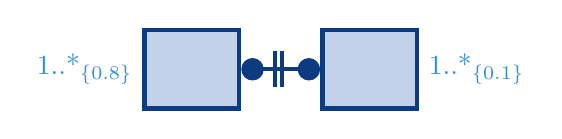
\begin{tikzpicture}
        \node[task] (accept) {\accept};
        \node[task,right=of accept] (reject) {\reject};
        \node[pwords,left=0mm of accept] {1..*$_{\{0.8\}}$};
        \node[pwords,right=0mm of reject] {1..*$_{\{0.1\}}$};
        \draw[notcoexistence] (accept) -- (reject);
    \end{tikzpicture}
  }
\end{center}
This model contains two mutually exclusive activities, $\accept$ and $\reject$, and indicates that often (in $80\%$ of the cases) $\accept$ is selected, whereas rarely (in $10\%$ of the cases) $\reject$ is selected. This captures a form of probabilistic choice, which also implicitly contemplates that none of the two activities occurs. In fact, from this very simple model, we can infer the following conditions on satisfying logs:
\begin{compactenum}
\item The $\constraint{not-coexistence}$ constraint linking $\accept$ and $\reject$ is crisp, and consequently no trace in the log can contain both $\accept$ and $\reject$.
\item Point 1, combined with the probabilistic $\constraint{existence}$ constraint on $\accept$, means that a trace in the log has $0.8$ probability of containing $\accept$ (which means that $\reject$ will not occur), and $0.2$ probability of not containing $\accept$ (which means that $\reject$ may occur or not).
\item A similar line of reasoning can be applied to the existence of $\reject$, which must appear in $10\%$ of the traces in the log.
\end{compactenum}
All in all, combining all the constraints, we get that the $10\%$ of traces containing $\reject$ must be disjoint from the $80\%$ containing $\accept$. This implicitly means that in the remaining $10\%$ of the traces, none of the two activities occur.
\end{example}

The second example shows that a consistent \pdeclare model may become inconsistent by changing the values of probabilities.

\begin{example}
  \label{ex:inconsistent-prob}
  Consider again the \pdeclare diagram in Example~\ref{ex:consistent-prob}. Clearly, if we change to $1$ the constraint probabilities attached to the two $\constraint{existence}$ constraints, the model becomes identical to that in Example~\ref{ex:inconsistency}, consequently becoming inconsistent. More in general, the model becomes inconsistent whenever the sum of the two probabilities exceeds $1$. This witnesses that there must exist some traces in which both constraints are satisfied, which contradicts the fact that $\accept$ and $\reject$ should not coexist. More precisely, if we denote by $p_a$ and $p_r$ the probabilities attached to the two $\constraint{existence}$  constraints, then there is a probability $p_a+p_r-1$ of having a trace that contains both $\accept$ and $\reject$.  For example, if we set $p_a = 0.8$ and $p_r = 0.3$, we have that $10\%$ of the traces in the log should contain both $\accept$ and $\reject$, which is impossible given the fact that every trace in the log should satisfy $\constraint{not-coexistence}(\accept,\reject)$.
\end{example}

The last example shows that, as customary in models with uncertainty, it is misleading to just consider the probabilities attached to single constraints when one wants to assess the probability of satisfying all of them at once.

\begin{example}
  \label{ex:prob-interplay}
  Consider the following \pdeclare model:
  \begin{center}
  \resizebox{3.5cm}{!}{
    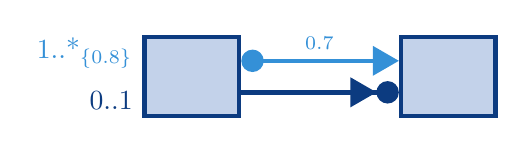
\begin{tikzpicture}[node distance=2cm]
      \node[task] (accept) {\accept};
      \node[pwords,left=0mm of accept,yshift=+3mm] {1..*$_{\{0.8\}}$};
      \node[left=0mm of accept,taskfg,yshift=-3mm] {0..1};

      \node[task,right=of accept] (pay) {\pay};
      \draw[response,pconstraint]
        ($(accept.east)+(0,2mm)$)
        -- node[above,pwords] {$_{\set{0.7}}$}
        ($(pay.west)+(0,2mm)$);
      \draw[precedence]
        ($(pay.west)-(0,2mm)$)
        --
        ($(accept.east)-(0,2mm)$);

    \end{tikzpicture}
  }
  \end{center}
  The model indicates that an order can be accepted at most once, and that often (in $80\%$ of the cases) it is actually accepted. In addition, it captures that with probability $0.7$ it is true that, whenever the order is accepted, then it is also consequently paid (multiple payment instalments are possible, by simply repeating the execution of $\pay$). Finally, payments are enabled only if the order has been previously accepted.

  By looking at the diagram, one could wrongly interpret that in $70\%$ of the cases it is true that the order is accepted and then paid. This is wrong because the $\constraint{response}(\accept,\pay)$ constraint can also be (vacuously) satisfied by a trace that does not contain at all occurrences of $\accept$. A natural question is then: what is the actual probability of observing traces that at some point contain $\accept$ and, later on, $\pay$ (possibly with other activity occurrences in between and afterward)? The answer is that this happens in half of the cases. To justify this non-trivial answer, one has to apply combined reasoning by considering the interplay of $\constraint{response}(\accept,\pay)$ and $\constraint{existence}(\accept)$, with their corresponding probabilities. More specifically, $\constraint{response}(\accept,\pay)$ can be satisfied in this model in two different ways:
  \begin{compactenum}
  \item by not executing at all $\accept$;
  \item by executing $\accept$ (which can be done only once, due to the presence of the crisp $\constraint{absence2}(\accept)$ constraint) and, later on, at least once $\pay$.
  \end{compactenum}
  These two situations, which we will call later on \emph{constraint scenarios}, should altogether cover exactly $70\%$ of the traces, as dictated by the constraint probability attached to $\constraint{response}(\accept,\pay)$. The first scenario must have probability $0.2$, because in $80\%$ of the traces $\accept$ must appear, as dictated by the $\constraint{existence}(\accept)$ constraint and its associated probability.
    But then, the second scenario, which is the one we are interested in, has probability $0.7-0.2 = 0.5$ (half of the traces in the log).
\end{example}

In the next section, we make the reasoning carried out in the discussed examples more systematic, showing how logical and probabilistic reasoning have to be combined towards a single, combined declarative framework.

%
\section{Reasoning on Time and Probabilities}
As we have seen in the previous section, to reason on conjunctions of probabilistic constraints, i.e., on \pdeclare models, we need to simultaneously take into account the temporal semantics of constraints and their associated probabilities.

Formally, this is done by relying on the probabilistic temporal logic over finite traces \PLTL, recently introduced in \cite{MaMP20}. More specifically, probabilistic constraints as defined here have a direct encoding into the fragment \PLTLz of \PLTL, also investigated in \cite{MaMP20}. We do not delve into the encoding, nor highlight the formal details on how to carry out this combined reasoning. We instead show algorithmically how to accomplish this, noticing that all the algorithmic techniques discussed next are correct thanks to \cite{MaMP20}. Again thanks to \cite{MaMP20}, we also get that, overall, the cost of reasoning on probabilistic constraints has the same complexity of reasoning with standard \LTLf constraints, i.e., \PS in the length of the constraints (this complexity bound is tight).


In the remainder of this section, we fix a \pdeclare model $\model = \tup{\tasks,\cset}$, where $\cset$ is partitioned into \emph{crisp constraints} $\crispc = \set{\tup{\varphi,p} \in \cset \mid p = 1}$ and (genuinely) \emph{probabilistic constraints} $\probc = \set{\tup{\varphi,p} \in \cset \mid p < 1}$. With a slight abuse of terminology, when we use the term ``crisp constraint'', we mean a constraint in $\crispc$, and, when we use the term  ``probabilistic constraint'', we mean a constraint in $\probc$. We also assume that $\crispc$ is a consistent \declare model, i.e., crisp constraints are satisfiable altogether. If not, then $\model$ has to be discarded, as it does not admit any conforming trace.


\subsection{Constraint Scenarios and Consistency of \pdeclare Models}
While crisp constraints must hold in every possible trace, probabilistic constraints may or may not hold (with a ratio specified by their probability). In addition, recall that when a constraint formula does not hold, then its negation must hold. Consequently, in the most general case, $\model$ is a compact description for the $2^{|\probc|}$ standard \declare models, each one obtained by considering all constraint formulae in $\crispc$, and by selecting, for each constraint $\tup{\varphi,p} \in \probc$, whether the constraint formula $\varphi$ or its complement $\neg \varphi$ is assumed to hold.

We call the so-obtained \declare models \emph{(constraint) scenarios}. To pinpoint a specific scenario, we fix an ordering over $\probc$, and we denote the scenario with a binary string of length $|\probc|$, where position number $i \in \set{1,\ldots,|\probc|}$ has value $1$ if the $i$-th probabilistic constraint in $\probc$ must hold, $0$ otherwise.

\begin{example}
  \label{ex:scenarios}
  Consider the \pdeclare model in Example~\ref{ex:prob-interplay}. By fixing the ordering over its probabilistic constraints where $\tup{\constraint{existence}(\accept),0.8}$ is first and $\tup{\constraint{response}(\accept,\pay),0.7}$ is second, we have the following $4$ scenarios:
  \begin{compactenum}
  \item Scenario $00$, where none of the two constraint formulae holds, and is consequently characterized by formula
  $\Box \neg \accept \land \Diamond (\accept \land \Box \neg \pay)$.
    \item Scenario $01$, where the $\constraint{response}$ constraint formula holds while the $\constraint{existence}$ one does not, and so has formula
  $\Box \neg \accept \land \Box (\accept \rightarrow \Diamond \pay)$.
    \item Scenario $10$, where the $\constraint{existence}$ constraint formula holds while the $\constraint{response}$ one does not, and so has formula
  $\Diamond \accept \land \Diamond (\accept \land \Box \neg \pay)$.
     \item Scenario $11$, where both formulae holds ($\Diamond \accept \land \Box (\accept \rightarrow \Diamond \pay)$).
  \end{compactenum}
\end{example}

Among the possible scenarios, only those that are logically consistent, i.e., are associated with a satisfiable formula, have to be retained. In fact, inconsistent scenarios do not admit any conforming trace. Obviously, when checking whether the scenario is consistent, its constraint formulae have to be conjoined with those in  $\crispc$.

\begin{example}
\label{ex:consistent-scenarios}
Consider the $4$ scenarios of Example~\ref{ex:scenarios}. Scenario $00$ has to be discarded because it is logically inconsistent: its formula $\Box \neg \accept \land \Diamond (\accept \land \Diamond \pay)$ is unsatisfiable (it is asking for the presence and absence of $\accept$). The other three scenarios are instead logically consistent.
\end{example}

\begin{example}
\label{ex:consistent-scenarios-2}
Consider the \pdeclare model in Example~\ref{ex:consistent-prob}. Also for this model there are $4$ scenarios, obtained by considering the two $\constraint{existence}$ constraints and their complements. The scenario where both constraints are not satisfied captures those traces where no decision is taken for the order, i.e., the order is not accepted nor rejected. The scenarios where one constraint is satisfied and the other is not account for those traces where a univocal decision is taken for the order. The scenario where both constraints are satisfied, thus requiring acceptance and rejection for the order, is inconsistent, due to the interplay of such constraints and the crisp $\constraint{not-coexistence}$ one. This corresponds to the standard \declare model of Example~\ref{ex:inconsistency}.
\end{example}

We have explicitly used the term \emph{logically} (in)consistent scenarios since there is no guarantee that these scenarios are actually plausible. This depends on their corresponding probabilities, which, in turn, are obtained by suitably combining the probabilities of their constitutive constraints in their positive or complemented form. This is done by enforcing the semantics of constraint probability, which requires to ensure the following: for every probabilistic constraint $\tup{\varphi,p}$, the sum of the probabilities assigned to those scenarios where $\varphi$ must hold must be equal to $p$.

To do so, we construct a system of linear inequalities whose variables represent the probabilities of possible scenarios \cite{MaMP20}. We denote such variables as $x_s$, where $s$ is the boolean string representing the scenario the variable is associated with. By considering a \pdeclare model $\model$, fixing $n = |\probc|$ and writing $i \in \set{0,\ldots,n-1}$ in binary, the system of inequalities $\Lmc_\model$ is:
\begin{align*}
x_i  &\geq  0  && 0\leq i < 2^n
  \tag{\text{$x_i$ are probabilities}} \\
 \sum_{i=0}^{2^n-1}x_i &= 1
  \tag{\text{$x_i$ are probabilities}}\\[2pt]
 \sum_{\text{$j$th position is 1}}x_i &= p_j &&  0\le j <n
  \tag{\text{constraint semantics}}\\
x_i &= 0 &&  \text{if scenario $i$ is logically inconsistent}
\end{align*}
Notably, $\Lmc_\model$ combines, at once, the logical and the probabilistic content of $\model$, on the one hand, imposing that the scenario probabilities agree with the constraint probabilities, and, on the other, forcing logically inconsistent scenario to have probability $0$.

 $\Lmc_\model$ may admit:
\begin{inparaenum}[\it (i)]
\item \emph{no solution}, witnessing that $\M$ is inconsistent;
\item \emph{one solution}, returning the exact probabilities for all the scenarios of $\M$,
\item \emph{multiple (possibly infinitely many) solutions}, witnessing that different probability distributions can be assigned to the scenarios.
\end{inparaenum} To obtain the ranges of probability for each scenario, one can turn the system of inequality into several optimizations problems where each probability variable is minimized and maximized.

It is worth noting that, when $\Lmc_\model$ is solvable, its solutions may force some scenario probabilities to be always equal to $0$. This witnesses the fact that even a logically consistent scenario may not have any conforming trace due to the interplay of constraint probabilities. We call \emph{plausible} those scenarios that have a probability $>0$.

\begin{example}
  Consider again the \pdeclare model in Example~\ref{ex:scenarios} with its 4 scenarios (one of which is logically inconsistent, as discussed in Example~\ref{ex:consistent-scenarios}). The four possible scenarios have corresponding probability variables $x_{00}$,  $x_{01}$, $x_{10}$ and $x_{11}$, constrained by the system of inequalities (we omit the fact that all variables are non-negative):
  $$
  \begin{array}{lclclclcl@{\qquad}l}
  x_{00} &+& x_{01} &+& x_{10} &+& x_{11} &=& 1 &
  \\
         & &        & & x_{10} &+& x_{11} &=& 0.8 &
  \text{semantics of $\tup{\constraint{existence}(\accept),0.8}$}
  \\
         & & x_{01} & &  &+&  x_{11}      &=& 0.7 &
  \text{semantics of $\tup{\constraint{response}(\accept,\pay),0.7}$}
  \\
  x_{00} & &       & &        & &         &=& 0 &
  \text{logical inconsistency of scenario $00$}
  \end{array}
  $$
The system admits a single solution, with $x_{00} = 0$, $x_{01} = 0.2$, $x_{10} = 0.3$ and $x_{11} = 0.5$, the last matching the informal discussion given in Example~\ref{ex:prob-interplay}.
\end{example}

We conclude the section with an informative \pdeclare model example that combines parts of the examples seen so far to capture a non-trivial fragment of an order-to-shipment process. We use parameters for constraint probabilities, then discussing the impact of grounding such probabilities to different actual values.

\begin{table}[t]
\caption{\label{tab:scenarios} Constraint scenarios of the \pdeclare model in Example~\ref{ex:running}, indicating whether they are logically consistent and, if so, providing the (shortest) conforming trace, and the scenario probability.}
{\scriptsize
\begin{tabularx}{\textwidth}{|C@{~~}C@{~~}C@{~~}C|c|l||c|}
\hline
\multicolumn{4}{|c|}{\textsc{scenario}} &
\textsc{logically} &
\multicolumn{1}{c||}{\textsc{shortest conforming}} &
\textsc{scenario}
\\
$\varphi_a$ &
$\varphi_r$ &
$\varphi_{ap}$ &
$\varphi_{ax}$ &
\textsc{consistent} &
\multicolumn{1}{c||}{\textsc{trace}} &
\textsc{probability}
\\
\hline
0 & 0 & 0 & 0 & N & & \\
\hline
0 & 0 & 0 & 1 & N &  & \\
\hline
0 & 0 & 1 & 0 & N &  & \\
\hline
0 & 0 & 1 & 1 & Y & empty trace & $1-p_a-p_r$\\
\hline
0 & 1 & 0 & 0 & N &  & \\
\hline
0 & 1 & 0 & 1 & N &  & \\
\hline
0 & 1 & 1 & 0 & N &  & \\
\hline
0 & 1 & 1 & 1 & Y & $\tup{\reject}$ & $p_r$\\
\hline
1 & 0 & 0 & 0 & Y & $\tup{\accept}$ & $2-p_a-p_{ap}-p_{ax}$\\
\hline
1 & 0 & 0 & 1 & Y & $\tup{\accept,\cancel}$ & $p_a+p_{ax}-1$\\
\hline
1 & 0 & 1 & 0 & Y & $\tup{\accept,\pay,\ship}$ & $p_a+p_{ap}-1$\\
\hline
1 & 0 & 1 & 1 & N &  & \\
\hline
1 & 1 & 0 & 0 & N &  & \\
\hline
1 & 1 & 0 & 1 & N &  & \\
\hline
1 & 1 & 1 & 0 & N &  & \\
\hline
1 & 1 & 1 & 1 & N &  & \\
\hline
\end{tabularx}
}


\end{table}

\begin{example}
  \label{ex:running}
Consider the following order-to-shipment \pdeclare  model:
    \begin{center}
  \resizebox{7cm}{!}{
    \begin{tikzpicture}[node distance=2cm]
      \node[task] (accept) {\accept};
      \node[pwords,above=0mm of accept] {1..*$_{\{p_a\}}$};
      \node[below=0mm of accept,taskfg] {0..1};

      \node[task,left = of accept] (reject) {\reject};
      \node[pwords,above=0mm of reject] {1..*$_{\{p_r\}}$};

      \draw[notcoexistence] (reject) -- (accept);


      \node[task,right=of accept] (pay) {\pay};

      \draw[response,pconstraint]
        ($(accept.east)+(0,2mm)$)
        -- node[above,pwords] {$_{\set{p_{ap}}}$}
        ($(pay.west)+(0,2mm)$);

      \draw[precedence]
        ($(pay.west)-(0,2mm)$)
        --
        ($(accept.east)-(0,2mm)$);



      \node[task,below=1cm of pay] (cancel) {\cancel};

      \draw[precedence,fill=white]
        ($(cancel.west)-(0,1.5mm)$)
        -|
        ($(accept.south east)-(3mm,0)$);

      \draw[response,pconstraint,fill=white]
        ($(accept.south east)-(1mm,0)$)
        |- node[above right,pwords] {$_{\set{p_{ax}}}$}
        ($(cancel.west)+(0,1.5mm)$)
        ;

      \draw[notcoexistence] (pay) -- (cancel);

       \node[task,right=of pay] (ship) {\ship};
       \draw[precedence]
        ($(ship.west)-(0,2mm)$)
        --
        ($(pay.east)-(0,2mm)$);
        \draw[response]
        ($(pay.east)+(0,2mm)$)
        --
        ($(ship.west)+(0,2mm)$);


    \end{tikzpicture}
  }
  \end{center}

To construct the $16$ possible scenarios for this model, the following constraints and \LTLf formulae have to be considered:
\begin{compactitem}[$\bullet$]
\item $\constraint{existence}(\accept)$ with formula $\varphi_a = \Diamond \accept$, and its complement $\Box \neg \accept$;
\item $\constraint{existence}(\reject)$ with formula $\varphi_r = \Diamond \reject$, and its complement $\Box \neg \reject$;
\item  $\constraint{response}(\accept,\pay)$ with formula $\varphi_{ap} = \Box( \accept \rightarrow \Diamond \pay)$,  and its complement $\Diamond(\accept \land \Box \neg \pay)$;
\item $\constraint{response}(\accept,\cancel)$ with formula $\varphi_{ax} = \Box( \accept \rightarrow \Diamond \cancel)$, and its complement $\Diamond(\accept \land \Box \neg \cancel)$.
\end{compactitem}

Table~\ref{tab:scenarios} summarizes the different constraint scenarios, their logical consistency and, in the last column, their probabilities computed by constructing and solving the system of inequalities described above.
Table~\ref{tab:cases} shows instead three different groundings for the constraint probability parameters and their impact on the probabilities of the scenarios. In particular, \emph{Case 1} is so that all the logically consistent scenarios may actually occur, even though with different probabilities. The most likely scenario, accounting for half of the traces, captures the happy path where the order is paid and shipped.
\emph{Case 2} assigns a different probability to $\constraint{response}(\accept,\cancel)$, causing scenario $1000$ to be not plausible anymore, being associated with probability $0$; intuitively, the interplay of constraints and their probabilities makes it impossible to just execute $\accept$ without taking further activities.
Finally, \emph{Case 3} increases the probability of $\constraint{response}(\accept,\cancel)$ even more, resulting in an inconsistent model.





\end{example}

\begin{table}[t]
\caption{\label{tab:cases} Three different groundings for the constraint probabilities used in the \pdeclare model in Example~\ref{ex:running}, and their impact on the scenario probabilities.}
{
\scriptsize
\begin{tabularx}{\textwidth}{|C@{~~}C@{~~}C@{~~}C|C|C|C|}
\hline
\multicolumn{4}{|c|}{\textsc{consistent scenario}} &
\textsc{case1} &
\textsc{case2} &
\textsc{case3}
\\
$\varphi_a$ &
$\varphi_r$ &
$\varphi_{ap}$ &
$\varphi_{ax}$ &
\scriptsize{
  $\begin{array}{@{}r@{~}l@{}}
      p_a =& 0.8\\
      p_r =& 0.1\\
      p_{ap} =& 0.7\\
      p_{ax} =& 0.3
  \end{array}$
  }
&
\scriptsize{
  $\begin{array}{@{}r@{~}l@{}}
      p_a =& 0.8\\
      p_r =& 0.1\\
      p_{ap} =& 0.7\\
      p_{ax} =& 0.5
    \end{array}$
  }
 &
\scriptsize{
  $\begin{array}{@{}r@{~}l@{}}
      p_a =& 0.8\\
      p_r =& 0.1\\
      p_{ap} =& 0.7\\
      p_{ax} =& 0.7
    \end{array}$
  }\\
\hline
0 & 0 & 1 & 1 & 0.1 & 0.1 &  \\
\cline{1-6}
0 & 1 & 1 & 1 & 0.1 & 0.1 & \\
\cline{1-6}
1 & 0 & 0 & 0 & 0.2 & 0 & inconsistent\\
\cline{1-6}
1 & 0 & 0 & 1 & 0.1 & 0.3 & \\
\cline{1-6}
1 & 0 & 1 & 0 & 0.5 & 0.5 &\\
\hline
\end{tabularx}
}
\end{table}






%\section{Reasoning with Constraint Scenarios}
Constraint scenarios can be used to perform a variety of tasks. We focus here on two fundamental ones: conformance checking and probabilistic constraint entailment.

\subsection{Conformance Checking}
In \declare, the simplest form of conformance checking amounts to check whether a given execution trace satisfies all constraints contained in the model, thus returning a yes/no answer.

In \pdeclare, this notion can be refined by considering the different constraint scenarios and their probabilities. Let $\M = \tup{\tasks,\cset}$ be a \pdeclare model, and $\tau$ be a trace over $\tasks$. The plausible scenarios of $\M$ are pairwise disjoint subsets of the overall set $\tasks^*$ of traces over $\tasks$. Disjointness comes from the fact that every pair of plausible scenarios is so that they disagree about at least one constraint, and no trace can conform with both of them. The complement of the traces accepted by the plausible scenarios then characterizes those traces that are not conforming with $\M$. To assess conformance, we can then proceed as follows:
\begin{inparaenum}[(1)]
\item Check $\tau$ against every plausible scenario of $\M$.
\item If one plausible scenario is so that $\tau$ holds there, output \emph{yes} together with the probability (or range of probabilities) attached to that scenario; the scenario probability gives an indication on whether the trace represents a ``mainstream'' execution of the process, or is instead an outlier behavior.
\item If no such scenario is found, then output \emph{no}.
\end{inparaenum}

\begin{example}
  Consider the \pdeclare model captured by \emph{Case 1} in Table~\ref{tab:cases}. Trace $\tup{\accept,\cancel,\pay}$ does not conform with the model, since paying and canceling are mutually exclusive. Trace $\tup{\accept,\cancel}$ is instead conforming, as it satisfies scenario $1001$. Since this scenario is associated with probability $0.1$, the analyzed trace represents an outlier behavior. Finally, trace $\tup{\accept, \pay, \ship, \ship, \pay, \ship}$ represents a mainstream behavior since it conforms with the most likely scenario $1010$, with probability $0.5$.
\end{example}

\subsection{Constraint Entailment}
It is well-known that \declare and other declarative process modeling languages have the issue of \emph{hidden dependencies} \cite{MPVC11}, namely the fact that constraints may interact with each other in subtle ways. This becomes even more complex in the case of probabilistic constraints. In this light, it becomes crucial to be able to ascertain whether a constraint is implied by a given model. Checking constraint implication in \declare is very simple: this simply amounts to check whether the \LTLf formula of the model implies the given constraint. In the case of \pdeclare, we extend this approach by computing, for a given \LTLf formula, what is the probability with which it is implied by the \pdeclare model. This is done as follows:
\begin{inparaenum}[(1)]
\item Initialize the constraint probability range to $0,0$.
\item For every plausible scenario, check whether the scenario implies the formula of interest in the classical \LTLf sense; if so, update the constraint probability by summing its minimum and maximum to the minimum and maximum probability associated with the scenario.
\item Return the constraint probability range.
\end{inparaenum}

\begin{example}
  Consider again the \pdeclare model captured by \emph{Case 1} in Table~\ref{tab:cases}. We want to check to what extent the model implies that the order is eventually shipped ($\Diamond \ship$). Shipment only occur if a payment occurs before, and therefore this formula is implied only by scenario $1010$, consequently getting a probability of $0.5$.

  We are also interested in checking to what extent the model implies that the order is not rejected ($\neg \Diamond \reject$). This formula holds in all those scenarios where $\constraint{existence}(\reject)$ is false. Therefore, this formula is implied with probability $0.9$.

  Finally, consider the \LTLf constraint $\neg(\Diamond \cancel \land \Diamond \ship)$, expressing the mutual exclusion between \cancel\ and \ship. This constraint is implied with probability $1$, due to the presence of the two crisp constraints $\constraint{not-coexistence}(\cancel,\pay)$ and $\constraint{precedence}(\pay,\ship)$, which must hold in every possible scenario (including the plausible ones).
\end{example}







%\section{Discovering \pdeclare Models from Event Logs}
\label{sec:discovery}
We now show that \pdeclare models can be discovered from event data using, off-the-shelf, already existing techniques, with a quite interesting guarantee: that the discovered model is always consistent.
%
We use the standard notation $[\cdot]$ for multisets, and use superscript numbers to identify the multiplicity of an element in the multiset.

A plethora of different algorithms have been devised to discover \declare models from event data \cite{LMMR07,MaCV12,CiccioM15,DBLP:conf/caise/SchonigRCJM16}. In general, the vast majority of these algorithms adopt the following approach to discovery:
\begin{inparaenum}[(1)] 
\item  Candidate constraints are generated by analyzing the activities contained in the log. 
\item For each constraint, its \emph{support} is computed as the fraction of traces in the log where the constraint holds.
\item Candidate constraints are filtered, retaining only those whose support exceeds a given threshold. 
\item Further filters (e.g., considering the ``relevance'' of a constraint \cite{DMMM18}) are applied. 
\item The overall model is checked for satisfiability, operating with different strategies if it is not; this is necessary since constraints with high support, but less than $1$, may actually conflict with each other \cite{DMMM17}.
\end{inparaenum}
%
In this procedure, the notion of support is formalized as follows.
\begin{definition}
The \emph{support} of an \LTLf constraint $\varphi$ in an event log $\mathcal{L} = [\tau_1, \dots,  \tau_n]$ is
\begin{equation*}
\mathit{supp}_{\mathcal{L}}(\varphi) = \frac{\vert\mathcal{L}_{\varphi}\vert}{\vert \mathcal{L}\vert}, \text{ where }\mathcal{L}_{\varphi} = [\tau \in \mathcal{L} \mid \tau \models \varphi]
\end{equation*}
\end{definition}
%
By the semantics of probabilistic constraints, we can adopt this approach off-the-shelf to discover \pdeclare constraints: \emph{we just use the constraint support as its associated probability, with operator $=$}. In other words, if $\varphi$ is discovered with support $p$, we turn it into the probabilistic constraint $\tup{\varphi,p}$. When doing so, we can also relax step (3), e.g., to retain constraints with a very low support, implying that their negated versions have a very high support.

\begin{example}
  Consider $\L = [\tup{\activity{close},\activity{acc}}^7,\tup{\activity{close},\activity{ref}}^2,\tup{\activity{close},\activity{acc},\activity{ref}}^1]$, capturing the evolution of 10 orders, 7 of which have been closed and then accepted, 2 of which have been closed and then refused, and 1 of which has been closed, then accepted, then refused. The support of constraint \constraint{response}(\activity{close},\activity{acc}) is $8/10 = 0.8$, witnessing that 8 traces satisfy such a constraint, whereas 2 violate it. This corresponds exactly to the interpretation of probability $0.8$ for the probabilistic \constraint{response}(\activity{close},\activity{acc}) constraint in Figure~\ref{fig:scenarios}. More in general, the entire \pdeclare model of Figure~\ref{fig:scenarios} can be discovered from $\L$ by considering the 6 constraints contained in that model and their corresponding support over $\L$.
\end{example}

A second key observation is that once this procedure is used to discover \pdeclare constraints, step (5) is unnecessary: the overall discovered model is in fact guaranteed to be satisfiable (in our probabilistic sense).
%
\begin{theorem}
Let $\Sigma$ be a set of activities, $\mathcal{L}$ be an event log over $\Sigma$,
and
$\mathcal{C}=\set{\tup{\varphi_1,p_1},\ldots,\tup{\varphi_n,p_n}}$ be a set of probabilistic constraints discovered from $\mathcal{L}$, such that for each $i \in \set{1,\ldots,n}$, $p_i = \mathit{supp}_{\mathcal{L}}(\varphi_i)$.
 The \pdeclare model $\tup{\Sigma,\mathcal{C}}$ is satisfiable.
\end{theorem}
%
\begin{proof}
Recall that $\tup{\Sigma,\mathcal{C}}$ is satisfiable if its corresponding \PLTLz formula
$\Phi:=\{\prob{p_1}\varphi_1,\ldots,\prob{p_n}\varphi_n\}$ is satisfiable.
To show this, we simply use $\mathcal{L}$ to build a model of $\Phi$.
%
For every set $I\subseteq \{1,\ldots,n\}$, let
$\varphi_I$ be the $\text{LTL}_f$ formula
\[
\varphi_I := \bigwedge_{i\in I} \varphi_i \land \bigwedge_{i\notin I}\neg\varphi_i,
\]
and let $\mathcal{L}_I$ be the sublog of $\mathcal{L}$ containing all the traces that satisfy $\varphi_I$. Note
that the sublogs $\mathcal{L}_I$ form a partition of $\mathcal{L}$; that is, every trace appears in exactly one
such $\mathcal{L}_I$.
%%
For each $I$ such that $\mathcal{L}_I$ is not empty, choose a representative $t_I\in\mathcal{L}_I$ and let
$p_I:=\frac{\vert \mathcal{L}_I \vert}{\vert \mathcal{L} \vert}$ be the fraction of traces that belong to $\mathcal{L}_I$. 
We build a stochastic language $\rho$ by setting $\rho(t_I)=p_I$ for each $I$ such that $\mathcal{L}_I\not=\emptyset$
and $\rho(\tau)=0$ for all other traces. We need to show that $\rho$ satisfies $\mathcal{C}$.
%%
Consider a constraint $\left<\varphi,p\right>\in\mathcal{C}$; we need to show that $\sum_{\tau\models\varphi}\rho(\tau)=p$.
Note that by construction, $\sum_{\tau\models\varphi}\rho(\tau)=\sum_{t_I\models\varphi}p_I$ and
since $\mathcal{L}_I$ form a partition the latter is in fact the fraction of traces that satisfy
$\varphi$. On the other hand, $p$ is also the
support of $\varphi$; that is, the proportion of traces satisfying $\varphi$. Hence, both values are equal, and $\rho$
satisfies the \pdeclare model.
\qed
\end{proof}
By this theorem, probabilistic constraints can be discovered in a \emph{purely local} way, having the guarantee that they will never conflict with each other. Obviously, non-local filters can still prove useful to prune implied constraints and select the most relevant ones.
Also, note that the probabilities of the discovered constraints can be easily adjusted when new traces are added to the log, by incrementally recomputing the support values after checking how many new traces satisfy the various constraints.

%The main open question related to the discovery of probabilistic constraints, which we intend to tackle in future work, is to determine when to stop the discovery procedure, and what is the impact of retaining constraints with various degrees of support in terms of over/under-fitting. 
%\newcommand{\formula}[1]{\mathit{formula}(#1)}
\newcommand{\probability}[1]{\mathit{prob}(#1)}

\section{Monitoring Probabilistic Constraints}
\label{sec:monitoring}
In Section~\ref{sec:scenarios}, we have shown how we can take a \pdeclare model and generate its constraint scenarios, together with their corresponding probability intervals. We now describe how this technique can be directly turned into an operational probabilistic monitoring and conformance checking framework.

Let $M = \tup{\Sigma,\mathcal{C}}$ be a \pdeclare model with $n$ probabilistic constraints. For simplicity, we do not distinguish between crisp and genuinely probabilistic constraints, nor prune away implausible scenarios: the produced monitoring results do not change, but obviously our implementation, presented at the end of this section, takes into account these aspects for optimization reasons.
%
$M$ generates $2^n$ constraint scenarios. As discussed in Section~\ref{sec:scenarios}, each scenario $S$ comes with a corresponding characteristic \LTLf formula, which amounts to the conjunction of positive and negated constraints in $\mathcal{C}$, where the decision of which ones are taken positive and which negative is defined by the scenario itself. We denote such a formula by $\formula{S}$. For example, if $\mathcal{C} = \set{\tup{\varphi_1,p_1},\tup{\varphi_2,p_2},\tup{\varphi_3,p_3}}$,  then $\formula{S_{101}}=\varphi_1 \land \neg \varphi_2 \land \varphi_3$.
%
In addition, each scenario $S$ comes with its probability interval, calculated by minimizing and maximizing its probability variable in the system of inequalities $\Lmc_M$. We denote such a probability interval by $\probability{S}$. From Example \ref{ex:intervals}, we have, e.g., that $\probability{S_{10}}= [0.7,0.8]$.

Since the characteristic formula of a scenario is in standard $\LTLf$, we can construct a \emph{scenario monitor} by recasting well-known techniques \cite{MMWV11,DDGM14}. Specifically, given an $\LTLf$ formula $\varphi$ over a set $\Sigma$ of activities, and a partial trace $\tau$ representing an ongoing process execution, a monitor outputs one of the four following truth values:
\begin{compactitem}[$\bullet$]
\item $\tau$ \emph{(permanently) satisfies} $\varphi$, if $\varphi$ is currently satisfied ($\tau \models \varphi$), and $\varphi$ stays satisfied no matter how the execution continues, that is, for every possible continuation trace $\tau'$ over $\Sigma$, we have $\tau \cdot \tau' \models \varphi$ (the $\cdot$ operator denotes the concatenation of two traces);
\item $\tau$ \emph{possibly satisfies} $\varphi$, if $\varphi$ is currently satisfied ($\tau \models \varphi$), but $\varphi$ may become violated in the future, that is, there exists a continuation trace $\tau'$ over $\Sigma$ such that $\tau \cdot \tau' \not\models \varphi$;
\item $\tau$ \emph{possibly violates} $\varphi$, if $\varphi$ is currently violated ($\tau \not\models \varphi$), but $\varphi$ may become satisfied in the future, that is, there exists a continuation trace $\tau'$ over $\Sigma$ such that $\tau \cdot \tau' \models \varphi$;
\item $\tau$ \emph{(permanently) violates} $\varphi$, if $\varphi$ is currently violated ($\tau \not\models \varphi$), and $\varphi$ stays violated no matter how the execution continues, that is, for every possible continuation trace $\tau'$ over $\Sigma$, we have $\tau \cdot \tau' \not\models \varphi$.
\end{compactitem}
In \cite{MMWV11,DDGM14}, it is shown that a monitor producing such outputs can be seamlessly obtained by constructing and determinizing the finite-state automaton $\aut_\varphi$ for $\varphi$, and assigning each automaton state to one of the four truth values.

\input{monitor}
\begin{figure*}[t!]
	\centering	
		\begin{tabular}{ c  c  }
			\makecell{			
				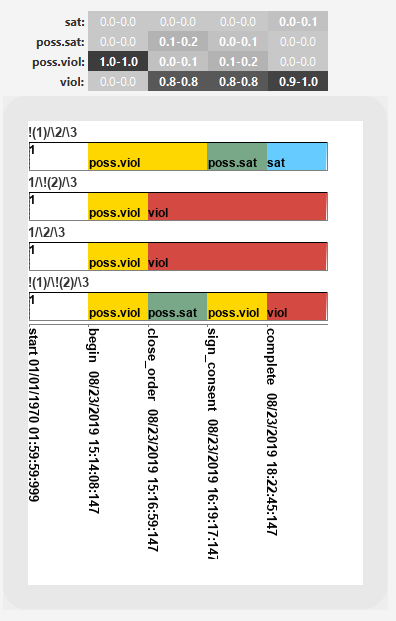
\includegraphics[width=0.5\textwidth]{images/LTL2Automaton_01_log_c_r.png}			
			}
			&
			\makecell{		
				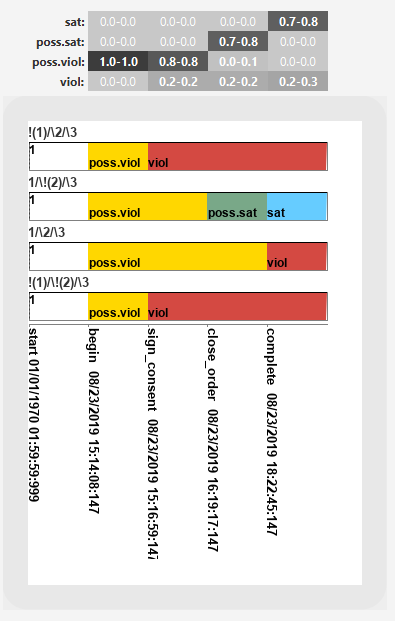
\includegraphics[width=0.5\textwidth]{images/LTL2Automaton_01_log_r_c.png}			
			} \\
			 trace $\tup{\activity{close},\activity{sign}}$ & trace $\tup{\activity{sign},\activity{close}}$
		\end{tabular}
	\caption{Output of the implemented tool on the example in \figurename\ref{fig:scenarios-2}.}
	\label{fig:ex0t1}
\end{figure*}

We proceed as follows. For each plausible constraint scenario $S$ over $M$, we construct the finite-state automaton $\aut_{\formula{S}}$, and turn it into a monitor as described above.\footnote{Implausible scenarios are irrelevant, since they produce an output that is associated to probability $0$, and would be therefore discarded when computing the aggregated probability intervals.} We then track the evolution of a running trace by delivering its events to \emph{all} such monitors in parallel, returning the truth values they produce. Note that, at runtime, we do not know in which scenario the trace will fall when completed. Hence, we actually do not know the exact truth value of the trace. For this reason, we compute the truth value of the trace probabilistically by aggregating the probabilities of the scenarios that produce the same truth value. In particular, we compute the \emph{aggregated probability interval} for each truth value, by taking the system of inequalities $\Lmc_M$ and calculating the extreme values of the aggregated interval by minimizing/maximizing the sum of the probability variables associated to the scenarios that produce that truth value. The aggregated probabilities give an indication of how probable it is that the trace can be associated to each specific truth value.

When a trace ends (which is signalled by a special, \emph{complete} event) all monitors currently outputting \emph{possible satisfaction} turn to \emph{permanent satisfaction}, and those outputting \emph{possible violation} turn to \emph{permanent violation}. Hence, when a trace ends, it either permanently violates all scenarios (thus being classified as a non-conforming one), or permanently violates all scenarios but one, which is permanently satisfied and consequently witnesses that the trace belongs to that scenario. Notably, this can be instrumental to classify traces into process variants.

%Interestingly, all monitors may agree on violation outputs, witnessing the non-conformance of the monitored trace. If, instead, monitors produce different outputs, their corresponding aggregated probabilities give a probabilistic indication of conformance that depends on how likely it is for the monitored trace to belong to the different plausible scenarios. The more the trace evolves, the more it becomes clear to which scenario it belongs, and in turn whether it configures itself as a common trace (belonging to a highly plausible scenario) or as an outlier one (belonging to a less plausible scenario).


\begin{example}
  Consider the \pdeclare model in Figure~\ref{fig:scenarios} with its three plausible scenarios (recall that four scenarios are logically plausible there, but one of those has probability $0$, so only three remains to be monitored). Figure~\ref{fig:monitoring} shows the result produced when monitoring a trace that at some point appears to belong to the most plausible scenario, but in the end turns out to conform to the less plausible one. From the image, we can also clearly see that the trace consisting only of a close order activity would be judged as non-conforming, as it would violate all scenarios.
\end{example}

This probabilistic monitoring technique has been fully implemented.\footnote{\url{https://bitbucket.org/fmmaggi/probabilisticmonitor/src/master/}} For solving systems of inequalities, we use the Java based LP solver\footnote{\url{http://lpsolve.sourceforge.net/5.5/}}. The implementation comes with various optimizations. First, scenarios are computed by directly imposing that crisp constraints with probability $1$ must hold in their positive form in all scenarios. Second, only plausible scenarios are retained for monitoring. Third, the results obtained by minimizing and maximizing for aggregate probability variables are cached, to avoid solving multiple times the same problem.
\figurename \ref{fig:ex0t1} shows the output of the implemented monitoring tool on the example in \figurename \ref{fig:scenarios-2} and for two different traces.\footnote{In the screenshots, 1 and 2 represent the probabilistic constraints labeled with 1 and 2 in \figurename \ref{fig:scenarios-2}, whereas 3 represents the crisp constraint in the same example.} Here, the aggregated probability intervals are shown with a dark gray or light gray background depending on whether their midpoint is closer to 1 or to 0, respectively, thus giving an indication of the most probable truth values for the monitored trace. The first trace (on the left) is classified as belonging to scenario $S_{01}$ and is an outlier because this scenario has low probability (corresponding to a probability interval of $\probability{S_{01}}= [0.0,0.1]$). The second trace (on the right) is classified as belonging to the highly plausible scenario $S_{10}$ (corresponding to a probability interval of $\probability{S_{10}}= [0.7,0.8]$).






%\section{Conclusions}
\label{sec:conclusion}

We have studied how to enrich constraint-based process models with uncertainty, captured as the probability that a trace will conform with a constraint or not. We have discussed how this impacts the semantics of a constraint model, and how logical and probabilistic reasoning have to be combined to provide core services such as consistency and conformance checking, as well as probabilistic constraint entailment.

Notably, all the techniques presented in this paper can be directly grounded with existing tools: automata-based techniques for \LTLf to carry out logical reasoning, and off-the-shelf systems to solve systems of linear inequalities (and corresponding optimization problems) to handle probabilities.

In~\cite{DBLP:conf/bpm/Maggi2020}, beside a concrete implementation of the techniques presented in this paper, we investigate the application of probabilistic business constraints to process mining, not only considering standard problems like discovery, but also delving into online operational support and, in particular, probabilistic monitoring~\cite{DBLP:conf/fase/MaggiMA12}. 
%\input{sections/declarereasoning}


\bibliographystyle{splncs04}
\bibliography{bibliography2}
%,bibliography2,references,libraryFiltered,main,Bibliography-CDC,DiCiccio,biblio}


\end{document}
